\chapter{Genomic Location Effect}\label{gle}

The tendency for mutations to occur in closed \gls{chromatin} regions has been reported both in cancer and other mutagenesis processes \citep{Polak2015,Prendergast2007ChromatinGenome}. This is hypothetically because closed chromatin regions, despite being less exposed to mutagens, are harder for repair systems to reach \citep{Prendergast2007ChromatinGenome,Teng1997ExcisionSequences, Morse2002PhotoreactivationCerevisiae}. Based on the premise that different cell-types harbour different chromatin structures \citep{Kundaje2015IntegrativeEpigenomes}, it is reasonable to expect that when developed into tumours, mutations are allocated differently between different cell-types. This chapter shows further evidence, through a G-test of independence and the \gls{or} statistic, that in cancers, mutations do tend to occur in closed rather than open chromatin regions, with the exception of breast adenocarcinoma and rectal cell carcinoma. The degree at which this phenomenon occurs varies across cancer types. In addition, the chapter also uses the \gls{bootstrap} to confirm that \gls{gle} alone, without the chromatin status input, are significantly different in different cancers. 

\section{Mutation location is influenced by chromatin status}

\begin{figure}[ht!]
    \begin{subfigure}{.5\textwidth}
    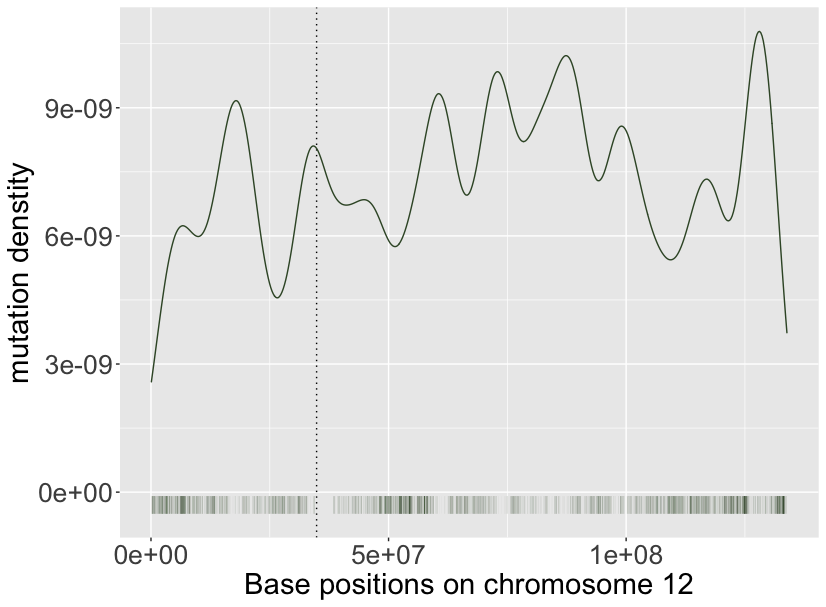
\includegraphics[width=\linewidth,height=0.7\textwidth]{graphics/mutdistribution_Skin-Melanoma.png}
    \caption{Skin-Melanoma}
    \label{fig:density_skin}
    \end{subfigure}
    ~
    \begin{subfigure}{.5\textwidth}
    
    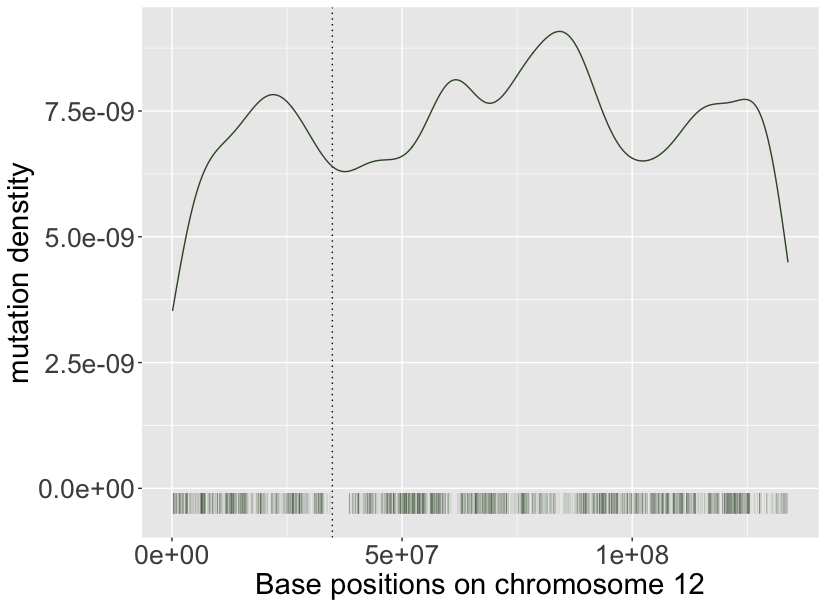
\includegraphics[width=\linewidth,height=0.7\textwidth]{graphics/mutdistribution_Kidney-RCC.png}
    \caption{Kidney-RCC}
    \label{fig:density_kidney}
    \end{subfigure} \\
    \vspace{0.5cm}
    
    \begin{subfigure}{.5\textwidth}
    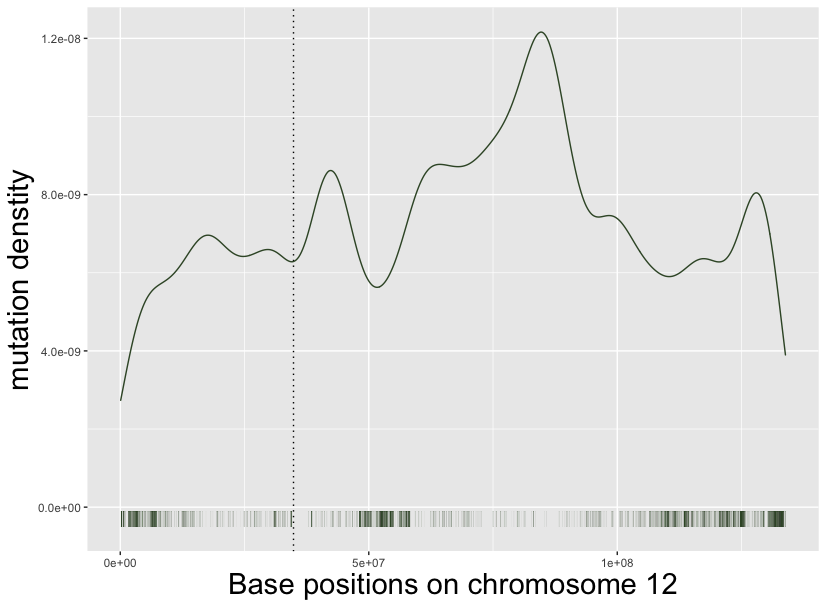
\includegraphics[width=\linewidth,height=0.7\textwidth]{graphics/mutdistribution_Liver-HCC.png}
    \caption{Liver-HCC}
    \label{fig:density_liver}
    \end{subfigure}
    ~
    \begin{subfigure}{.5\textwidth}
    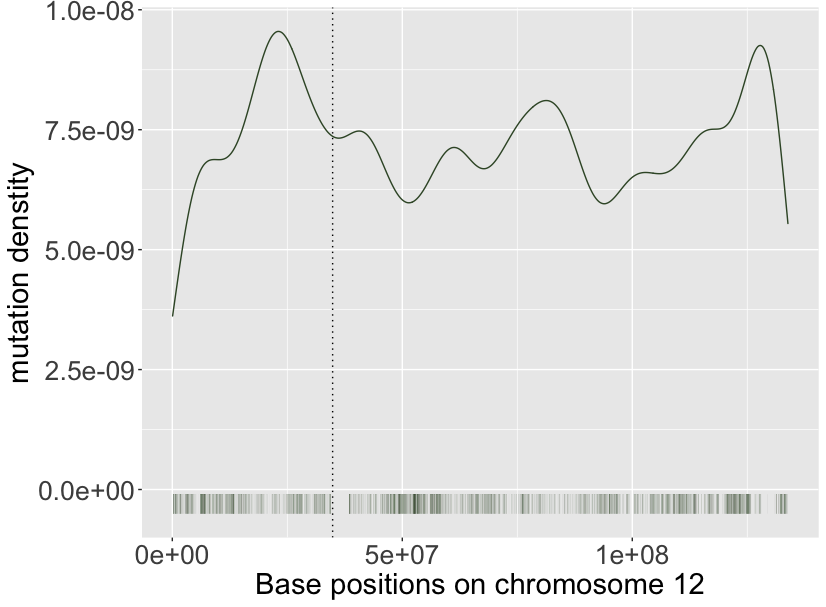
\includegraphics[width=\linewidth,height=0.7\textwidth]{graphics/mutdistribution_Panc-AdenoCA.png}
    \caption{Panc-AdenoCA}
    \label{fig:density_panc_adenoca}
    \end{subfigure} \\
    \caption{\textbf{Mutations tend to be found in closed chromatin regions.} Different cancers differ in the distribution of mutations across the genome. Here chromosome 12 is shown. (a) Skin-Melanoma (b) Kidney-RCC (c) Liver-HCC (d) Panc-AdenoCA, the other cancers are shown in Figure \ref{fig:apdx_mutation_density}. The shaded bars below the x-axis indicate open chromatin regions, the gaps indicate closed chromatin regions of the original cell types. The vertical dotted line indicates the position of the centromere.}
    \label{fig:mutation_density}
\end{figure}

\section{GLE is significantly different for different cancers}